\subsection{传统SIR模型}
\citeauthor{对流行病数学理论的贡献}在\citeyear{对流行病数学理论的贡献}年研究黑死病时提出了仓室模型,模型中将人口分为三类:
\begin{itemize}
	\item 易感者(susceptibles),$S$人群
	\item 感染者(infectives),$I$人群
	\item 康复者(recovered),$R$人群
\end{itemize}
\par 根据其人群划分将其称为$SIR$
\cite{对流行病数学理论的贡献}模型。
\par $SIR$模型的建立基于几个假设\cite{对流行病数学理论的贡献}:
\begin{itemize}
	\item 人口总数保持常量(包含死亡人数)
	\item 单位时间$t$传染人数与$S$和$I$人数成正比,即$S\to I = \alpha SI$
	\item 单位时间$t$康复人数与$I$成正比,即$I\to R = \beta I$
\end{itemize}
\subsubsection{符号表}
\begin{table}[H]
	\centering
	\caption{SIR模型符号表}
	\label{table:SIR模型符号表}
	\begin{tabular}{ll}
		\hline
		符号     & 含义                     \\
		\hline
		S        & 易感者                   \\
		I        & 感染者                   \\
		R        & 康复者                   \\
		$\alpha$ & $S$群体变为$I$群体的概率 \\
		$\beta$  & $I$群体变为$R$群体的概率 \\
		\hline
	\end{tabular}
\end{table}
\subsubsection{模型}
\par 感染机制如下:
\begin{align}
	S(t) & \xrightarrow \alpha I(t) \\
	I(t) & \xrightarrow \beta R(t)
\end{align}
可以用积分方程表示为
\begin{align}
	\dt{S} & = -\alpha SI          \\
	\dt{I} & = \alpha SI - \beta I \\
	\dt{R} & = \beta I
\end{align}
\subsection{对于模型表述方式的讨论}
\par 经典SIR模型的表述方式简洁直观,但在扩建模型时会产生一些问题:
由表\ref{table:SIR模型符号表}可预见,随着划分人群的增多,人群间感染机制也随之复杂,不同人群之间转变率的符号也会增多或者改变含义,这会使读者对符号的理解产生负面的路径依赖影响,对于模型的扩建是十分不利的。
\par 本文将采用另一种较为抽象的模型表述方式,以此来减轻读者的思维负担。
\subsubsection{新的符号表}
\begin{table}[H]
	\centering
	\caption{新的SIR模型符号表}
	\begin{tabular}{ll}
		\hline
		符号       & 含义                              \\
		\hline
		S          & 易感者                            \\
		I          & 感染者                            \\
		R          & 康复者                            \\
		$\P{a}{b}$ & a群体变为b群体的概率              \\
		$\T{a}{b}$ & 单位时间$t$内a群体变为b群体的人数 \\
		\hline
	\end{tabular}
\end{table}
\par 将a到b群体的转换概率用$\P{a}{b}$表示,单位时间内a到b群体转变的人数为$\T{a}{b}$。
\subsubsection{新的模型表述}
\par 感染机制如下:
\begin{align}
	S(t)\xrightarrow{\P{S}{I}}I(t) \Rightarrow \TP{S}{I}{SI} \\
	I(t)\xrightarrow{\P{I}{R}}R(t) \Rightarrow \TP{I}{R}{I}
\end{align}
\par 可将其简化为:
\begin{align}
	\TP{S}{I}{SI} \\
	\TP{I}{R}{I}
\end{align}
\par 将所有人群放到一个集合$\mathbb{A}$中,则模型的积分方程为:
\begin{equation}
	\dt{a} = \sum\left(\T{b}{a}-\T{a}{b}\right)
\end{equation}
\par 其中$a\in\mathbb{A}$,$b\in\mathbb{A}$且$b\not=a$,不在感染机制中的$\T{a}{b}$为$0$。
\par 值得注意的是,该积分式对本文中提到的所有模型都适用,这意味着我们将不必再关心模型的积分式,只需关注模型新引入的群体及其引起的感染机制$\T{a}{b}$变化即可。
\par 现在,可以这样方便清晰的来描述$SIR$模型:
\begin{itemize}
	\item 人群
	      \subitem $S$:易感者
	      \subitem $I$:感染者
	      \subitem $R$:康复者
	\item 感染机制
	      \subitem
	      \begin{align}
		      \TP{S}{I}{SI} \\
		      \TP{I}{R}{I}
	      \end{align}
	      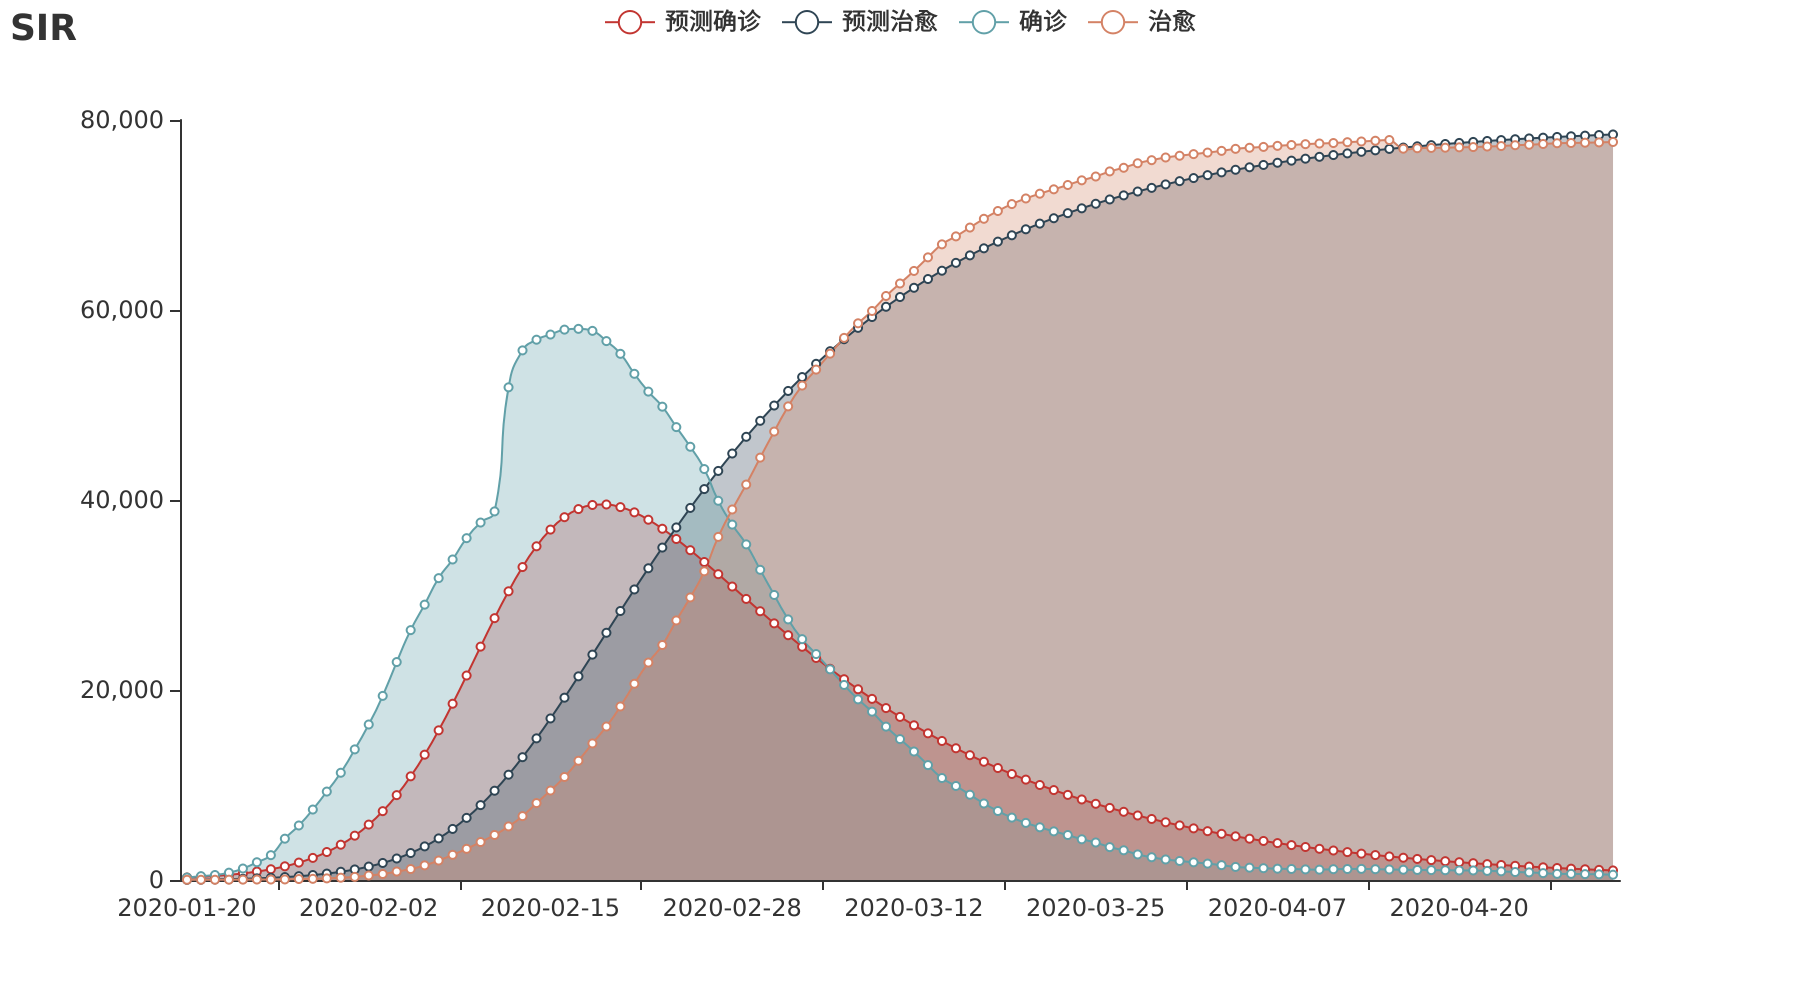
\includegraphics[scale=1]{SIR.eps}
\end{itemize}